\documentclass[border=3mm,tikz,preview]{standalone}
\usepackage[utf8]{inputenc}
\usepackage{amsmath,amssymb,amsfonts}
\usepackage{graphicx}
\usepackage{tikz}
\usetikzlibrary{shapes.geometric, arrows.meta, positioning, shadows, calc, fit, backgrounds}
\usepackage{xcolor}
\begin{document}

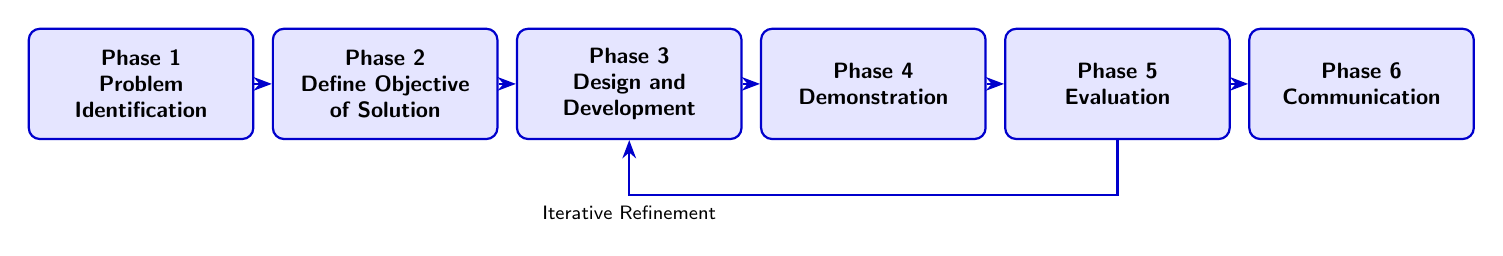
\begin{tikzpicture}[
    phase/.style = {rectangle, draw=blue!80!black, fill=blue!10!white, thick, rounded corners=4pt, align=center, font=\sffamily\bfseries\footnotesize, text width=2.5cm, minimum height=1.4cm, inner sep=5pt},
    arrow/.style = {draw=blue!80!black, ->, >=Stealth, thick}
]

\node (p1) [phase] at (0,0) {Phase 1\\Problem\\Identification};
\node (p2) [phase] at (3.1,0) {Phase 2\\Define Objective\\of Solution};
\node (p3) [phase] at (6.2,0) {Phase 3\\Design and\\Development};
\node (p4) [phase] at (9.3,0) {Phase 4\\Demonstration};
\node (p5) [phase] at (12.4,0) {Phase 5\\Evaluation};
\node (p6) [phase] at (15.5,0) {Phase 6\\Communication};

\draw [arrow] (p1) -- (p2);
\draw [arrow] (p2) -- (p3);
\draw [arrow] (p3) -- (p4);
\draw [arrow] (p4) -- (p5);
\draw [arrow] (p5) -- (p6);

% Clean Orthogonal Loop Arrow (No Overlap)
\draw [arrow] (p5.south) -- ++(0,-0.7) -| node[below,midway,font=\sffamily\scriptsize]{Iterative Refinement} (p3.south);

\end{tikzpicture}

\end{document}
